\documentclass{beamer}
\usecolortheme[RGB={0,102,51}]{structure}
\usetheme[height=9mm]{Rochester}
\usepackage{animate}

\usepackage{amsfonts,amssymb,amscd,amsmath,mathrsfs,amsthm}

\usepackage{tikz}
\usetikzlibrary{lindenmayersystems}
\pgfdeclarelindenmayersystem{A}{%
  \symbol{F}{\pgflsystemstep=0.6\pgflsystemstep\pgflsystemdrawforward}
  \rule{A->F[+A][-A]}
}
\usepackage{minted}
\usepackage{caption}
\usepackage{subcaption}


% Usetheme:
%
%\usetheme{Helsinki}

\author{Steven Glasford}
\title{Modeling a Fungal War on a Plant.}
\date{\today}
%\thanks{Dr. Ivan Yegorov}




\begin{document}

% Frame 1
\begin{frame}
\maketitle
\end{frame}
%todo: add background photo from https://bygl.osu.edu/sites/default/files/field/image/tar%20spot%20punctatum%203%20%20S%20Fair%208-20-16.jpg to the title page it has a good photo of fungal pathagen

\AtBeginSection[]  % A frame titled `Content' is added before every new section starts.
{
\begin{frame}<beamer>
\frametitle{Content} % Title of the automatically added frame
\tableofcontents[currentsection]   % List all the structure components that call this frame (section, subsection, subsubsection,...; add `current')
\end{frame}
}


% Section `Introduction'; sections are defined outside of frames. They may lead to the automatic inclusion of additional frames, see above.
\section{Introduction}
% \subsection{Motivation}
\begin{frame}{Pathogens are costly.}
    Pathogens make living things sick. \newline
    
    COVID-19 is a very important pathogen. \newline
    
    Pathogens can end up costing gigantic loses. \newline
    
    2016 alone saw \$540 billion in agricultural damages from plant pathogens. 
    
        
    \begin{center}
    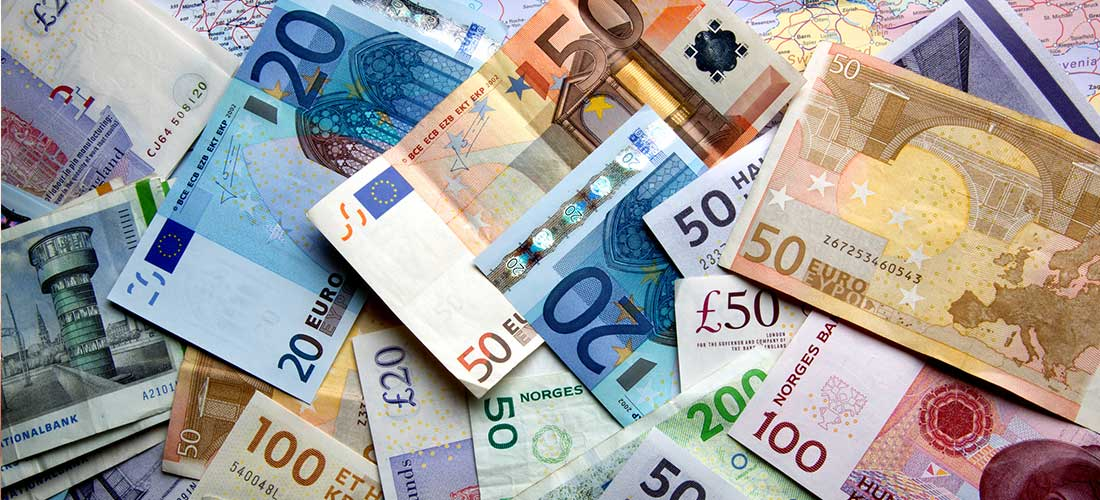
\includegraphics[ height = 4cm ]{money.jpg}
    \end{center}
\end{frame}

\begin{frame}{What is a fungal war?}
    We will be looking at parasitic pathogenic fungi, such as leaf rust or maple tar spots. \newline
    
    Limited resources, fighting for resources, not each other.\newline
    
    Host has finite resources, fungus wants to eat the leaf.
    
    \begin{center}
        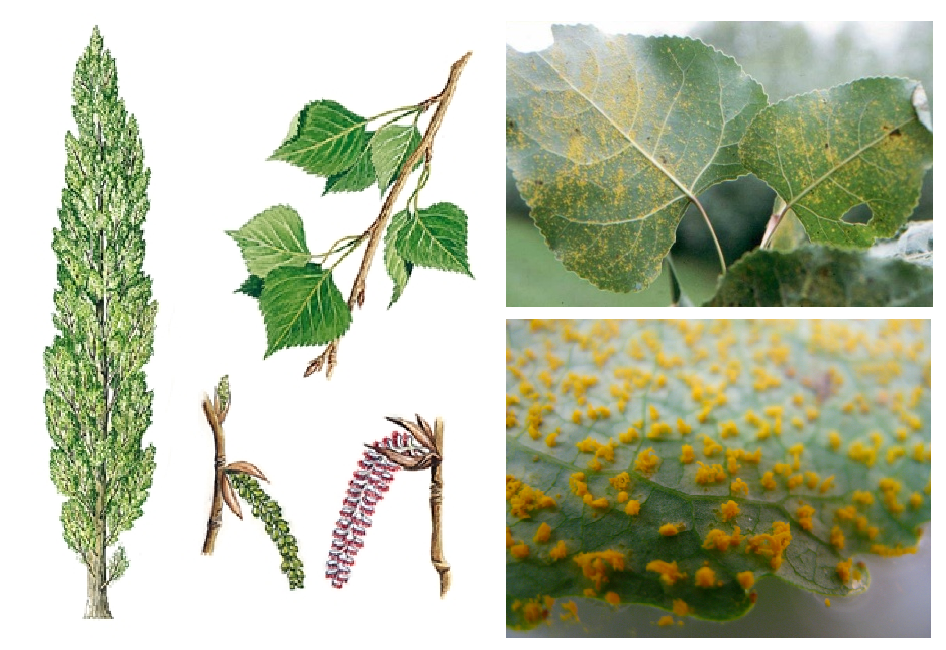
\includegraphics[ width = 7cm, height = 4.6cm ]{Figure_poplar_leaf_rust.pdf}
    \end{center}
\end{frame}

\begin{frame}{Closer inspection of Fungi}
    Pathogens in mind exploit leaf tissue. \newline

    Growth in the leaf is conducted using mycelia. \newline

    Spore production gets to more leaves.

    \begin{center}
        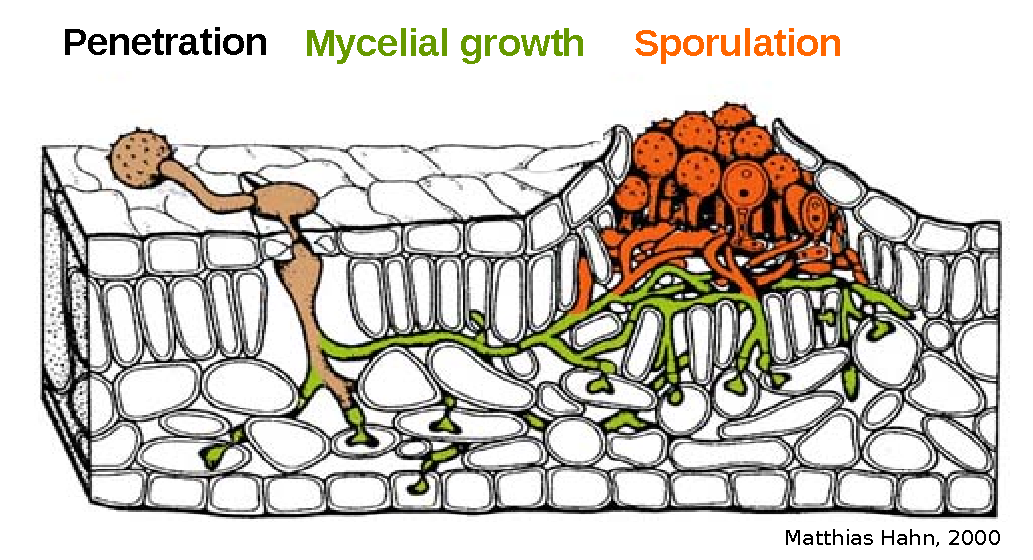
\includegraphics[ width = 9.5cm, height = 5cm ]{Figure_biotrophic_pathogens.pdf}
    \end{center}
\end{frame}

\section{Modeling}
% \subsection{Description}
\begin{frame}{Description of fungal equations.}
    We focus on a single season, on a single plant, without evolution. \newline
    
    Unrealistic in the wild (wild is complicated), we can still get useful results.

    \begin{center}
        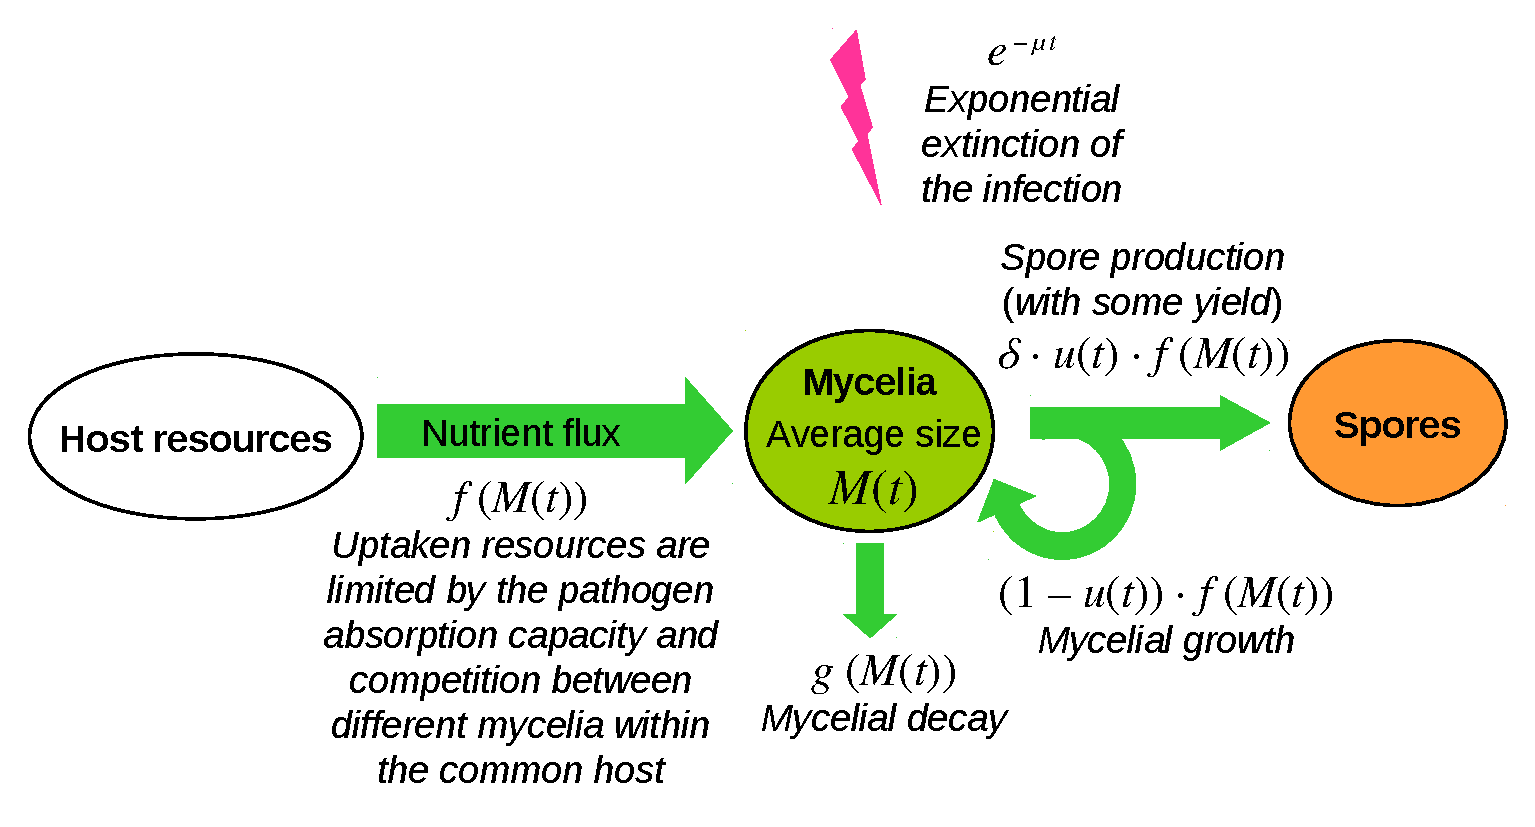
\includegraphics[ width = 10.5cm, height = 6cm ]{Figure_scheme.pdf}
    \end{center}
\end{frame}

% \subsection{Assumptions}
\begin{frame}{Convert to equations}
    Using the information from the previous slide we can get:
    
    $$ 
    \left\{ \begin{aligned}
    & \frac{d M_1(t)}{dt} \:\: = \:\: (1 - u_1(t)) \, f_1(M_1(t), M_2(t)) \: - \: g(M_1(t)), \\
    & \frac{d M_2(t)}{dt} \:\: = \:\: (1 - u_2(t)) \, f_2(M_1(t), M_2(t)) \: - \: g(M_2(t)), \\
    & f_i(M_1, M_2) \:\: \stackrel{\mathrm{def}}{=} \:\: \nu(n_1 M_1 \, + \, n_2 M_2) \: \rho(M_i), \quad i = 1,2, \\
    & 0 \leqslant u_i(t) \leqslant 1, \quad i = 1,2, \quad t \in I_T, \\
    & M_1(0) = M_1^0, \quad M_2(0) = M_2^0.
    \end{aligned} \right.
    $$
\end{frame}

\begin{frame}{Assumptions}
    $n$ is the lesion density and is constant. \newline
    
    The nutrient flux is represented as
    $$
    f(M) \: \stackrel{\mathrm{def}}{=} \: \nu(n M) \, \rho(M),
    $$
    where $\rho(M)$ is the amount of resources that flow through a single mycelium. $ \nu(n M) $ describes the negative influence of competing mycelia. \newline
    
    We will assume the resident is cohort 1, and the mutant is cohort 2.
\end{frame}

% \subsection{Equations}
\begin{frame}{Uninvadable strategies}
    The cohorts are not actually fighting each other, they are fighting for limited resources. \newline
    
    The war forms a zero-sum feedback game: resident defends, mutant is offensive. \newline
    
    We assume that the cohorts use uninvadable strategy, each cohort tries it's best and tries to ensure the other cohort does not fully invade. \newline
    
    An uninvadable strategy is also known as evolutionary stable strategy.
\end{frame}


% \subsection{Method of solving.}
\begin{frame}{Uninvadable equations}
    Let $ J_i $ be the marginal fitness (the amount of success of cohort $i$)
    $$J_i(u_1, u_2) = \: \int\limits_{I_T} u_i(t) f_i(M_1(t), M_2(t)) \, \delta \, e^{-\mu t} \, dt \: $$ of cohort~$ i $. \newline
    
    We can then say that the resident is not invaded if: $$ \: J(u_1, u_2) \: \stackrel{\mathrm{def}}{=} \: J_2(u_1, u_2) - J_1(u_1, u_2) \: \leqslant \: 0. $$ \newline
    
    We are most interested in modeling when $J$ forms a saddle point (ie $J = 0$).
    
\end{frame}

\begin{frame}{Differential Game}
    The previous slides gives us the following:
    $$
    \begin{aligned}
    & J(u_1(\cdot), u_2(\cdot)) \:\: = \:\: J_2(u_1(\cdot), u_2(\cdot)) \: - \: J_1(u_1(\cdot), u_2(\cdot)) \:\: = \\
    & = \:\: \int\limits_{I_T} (u_2(t) \, f_2(M_1(t), M_2(t)) \: - \: u_1(t) \, f_1(M_1(t), M_2(t))) \: \delta \, e^{-\mu t} \: dt \:\:
    \longrightarrow \\
    & \longrightarrow \:\: \inf_{u_1(\cdot)} \: \sup_{u_2(\cdot)} \:\: \mbox{or} \:\:
    \sup_{u_2(\cdot)} \: \inf_{u_1(\cdot)} \, ,
    \end{aligned}
    $$ 
    this describes how the first cohort tries t maximize its resistance to the second, and vice versa.\newline
    
    $\inf$ is the infimum (greatest) $\sup$ is the supremum (least).\newline
    
    $\inf\sup=\sup\inf$ describes a saddle point.
    
\end{frame}

\section{Execution and Code}
% \subsection{Code.}
\begin{frame}{Numerical Analysis}
    The equations we are working with are nonsmooth, making them difficult to solve exactly. \newline

    We use computers to simulate this system. \newline
    
    We can convert our equations into Hamilton--Jacobi--Isaac equation (HJI). \newline
    
    We can then solve the HJI with ROC-HJ (Reachability, Optimal Control, and Hamilton-Jacobi equations).
\end{frame}

\begin{frame}{Hamilton--Jacobi--Isaac equation}
    For brevity we exclude the reasoning behind converting to a Hamiltonian. Additional information can be found in \cite{YegorovGrognardMailleretHalkettBernhard2019}.\newline
    
    \begin{equation}
        \left\{ 
            \begin{aligned}
                & \frac{\partial V(t, M_1, M_2)}{\partial t} \: + \: \mathcal{H}
                \left( t, M_1, M_2, \frac{\partial V(t, M_1, M_2)}{\partial M_1},
                \frac{\partial V(t, M_1, M_2)}{\partial M_2} \right) \:\: = \:\: 0, \\
                & V(T, M_1, M_2) \: = \: 0, \\
                & t \in [0, T], \quad (M_1, M_2) \: \in \: G.
            \end{aligned} 
        \right.  
        \label{15}
    \end{equation}
\end{frame}

\begin{frame}{Resource Control Strategy}
    The Hamiltonian can be reduced to the following:
    \begin{equation}
        \begin{aligned}
            & u_1(t, M_1, M_2) \:\: = \:\: 
            \begin{cases}
                0, & e^{-\mu t} \: + \: \frac{\partial V(t, M_1, M_2)}{\partial M_1}
                 \: < \: 0, \\
                1, & e^{-\mu t} \: + \: \frac{\partial V(t, M_1, M_2)}{\partial M_1}
                \: > \: 0, \\
                \mbox{arbitrary from} \:\: [0, 1], & e^{-\mu t} \: + \: \frac{\partial
                V(t, M_1, M_2)}{\partial M_1} \: = \: 0,
            \end{cases} \\
            & u_2(t, M_1, M_2) \:\: = \:\: 
            \begin{cases}
                0, & e^{-\mu t} \: - \: \frac{\partial V(t, M_1, M_2)}{\partial M_2}
                \: < \: 0, \\
                1, & e^{-\mu t} \: - \: \frac{\partial V(t, M_1, M_2)}{\partial M_2}
                \: > \: 0, \\
                \mbox{arbitrary from} \:\: [0, 1], & e^{-\mu t} \: - \: \frac{\partial V(t,
                M_1, M_2)}{\partial M_2} \: = \: 0.
            \end{cases}
        \end{aligned}  
        \label{16}
    \end{equation}
    Where $u_1$ corresponds to the resource strategy for cohort 1 (resident), and $u_2$ corresponds to the strategy for cohort 2 (mutant)
\end{frame}

\begin{frame}{Reverse Time}
    ROC-HJ works backwards (enables user to start with an outcome and see how it started). \newline
    
    We must rewrite our equations in reverse.
    
    \begin{equation}
        \left\{ 
            \begin{aligned}
                & \frac{\partial V(T - \tau, M_1, M_2)}{\partial \tau}    \:\: + \:\:
                \max_{u_1 \in [0, 1]} \: \min_{u_2 \in [0, 1]} \:
                \left( -H \left( T - \tau, \, M_1, \, M_2, \, u_1, \, u_2, 
                {}^{{}^{{}^{{}^{{}^{}}}}} \right. \right. \\
                & \qquad\qquad\qquad\qquad\qquad
                \left. \left. \frac{\partial V(T - \tau, M_1, M_2)}{\partial M_1}, \,
                \frac{\partial V(T - \tau, M_1, M_2)}{\partial M_2}     \right) \right) \:\: =
                \:\: 0, \\
                & V(T - \tau, M_1, M_2) \left|_{\tau = 0} \right. \: = \: 0, \\
                & \tau \in [0, T], \quad (M_1, M_2) \: \in \: G,
            \end{aligned} 
        \right.  \label{75}
    \end{equation}
\end{frame}

\begin{frame}{Example and Basic Parameters}
    We use Finite Difference Method,\newline
    Second-order time discretization, \newline
    Find the saddle strategies.\newline
    
    ROC-HJ \cite{ROCHJ2019}.
    
    \begin{figure}[ht]
        \inputminted[
            frame=lines,
            framesep=2mm,
            baselinestretch=1.2,
            fontsize=\footnotesize,
            firstline=15, 
            lastline=17]{c}{code/data.h}
        \caption{Configurations of descriptive variables}
        \label{code:defaults}
    \end{figure}
\end{frame}

% \subsection{Output}
\begin{frame}{Output}
    ROC-HJ produces a large amount of data in .dat files.
    \begin{figure}[ht]
        \inputminted[
            frame=lines,
            framesep=2mm,
            baselinestretch=1.2,
            fontsize=\footnotesize,
            firstline=1, 
            lastline=5]{c}{code/VF20_100.dat}
        \caption{The first 5 lines from when $\tau=20$ produced from ROC-HJ.}
        \label{code:datfile}
    \end{figure}
    Describes the angle, and magnitude at a point, very large file 500k+ lines.\newline
    Needs to graphed to produce meaningful results.
\end{frame}

\section{Graphs and Analysis}
\begin{frame}{Graphs}
    \begin{figure}
    % \centering
    \begin{subfigure}{.48 \textwidth}
        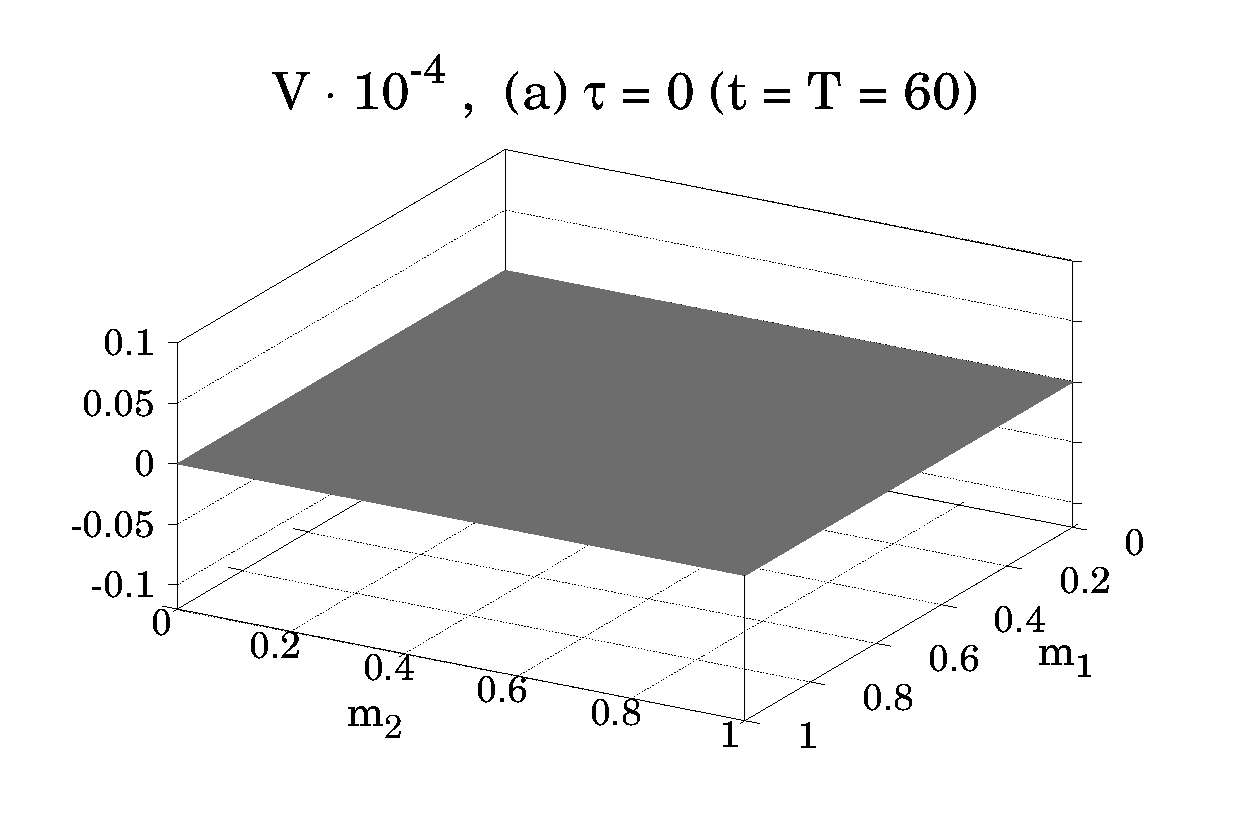
\includegraphics[width = \textwidth]{figures/Figure_4a.pdf}
        \caption{Strategies conducted at the end of the simulation.}
        \label{fig_4_a}
    \end{subfigure}
    \hfill
    \begin{subfigure}{.48 \textwidth}
        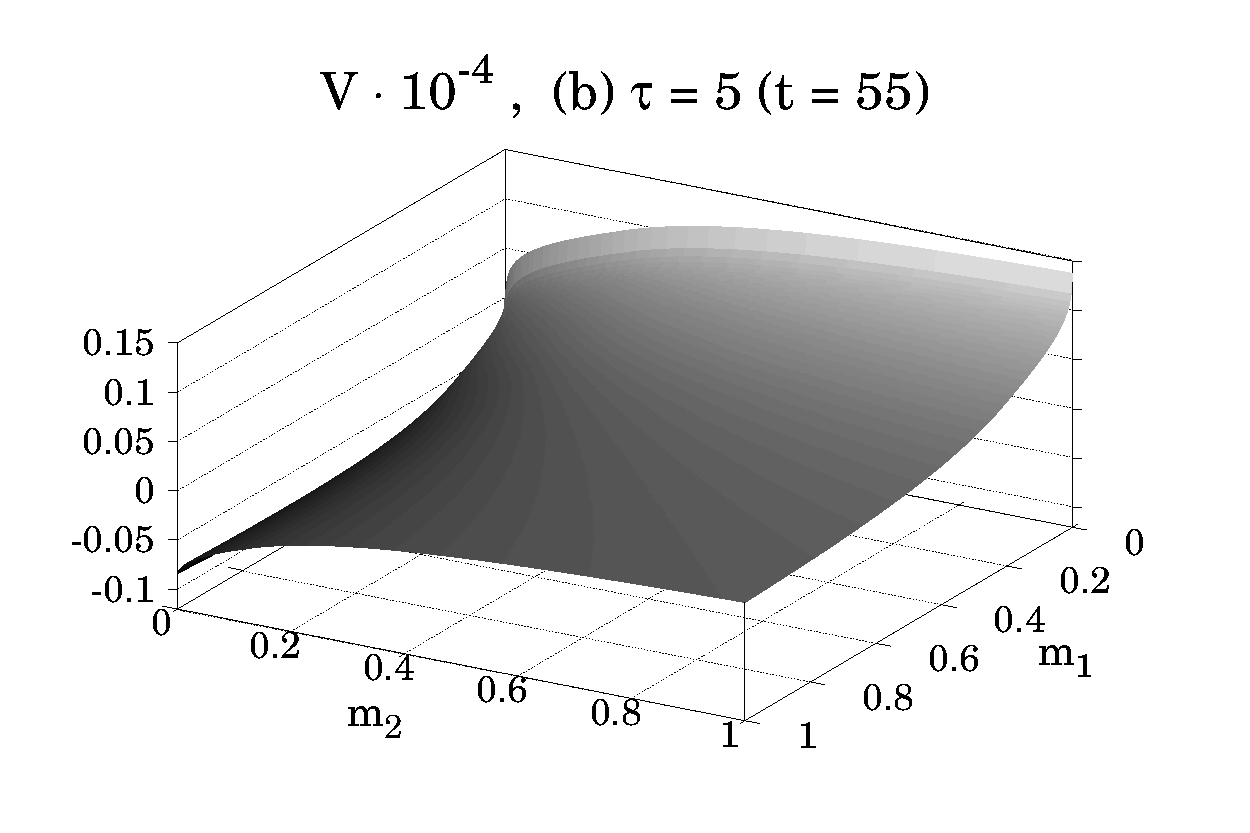
\includegraphics[width = \textwidth]{figures/Figure_4b_1.pdf}
        \caption{Competition between the fungi increases near the end of the simulation.}
        \label{fig_4_b}
    \end{subfigure}
    \hfill
    \begin{subfigure}{.48 \textwidth}
        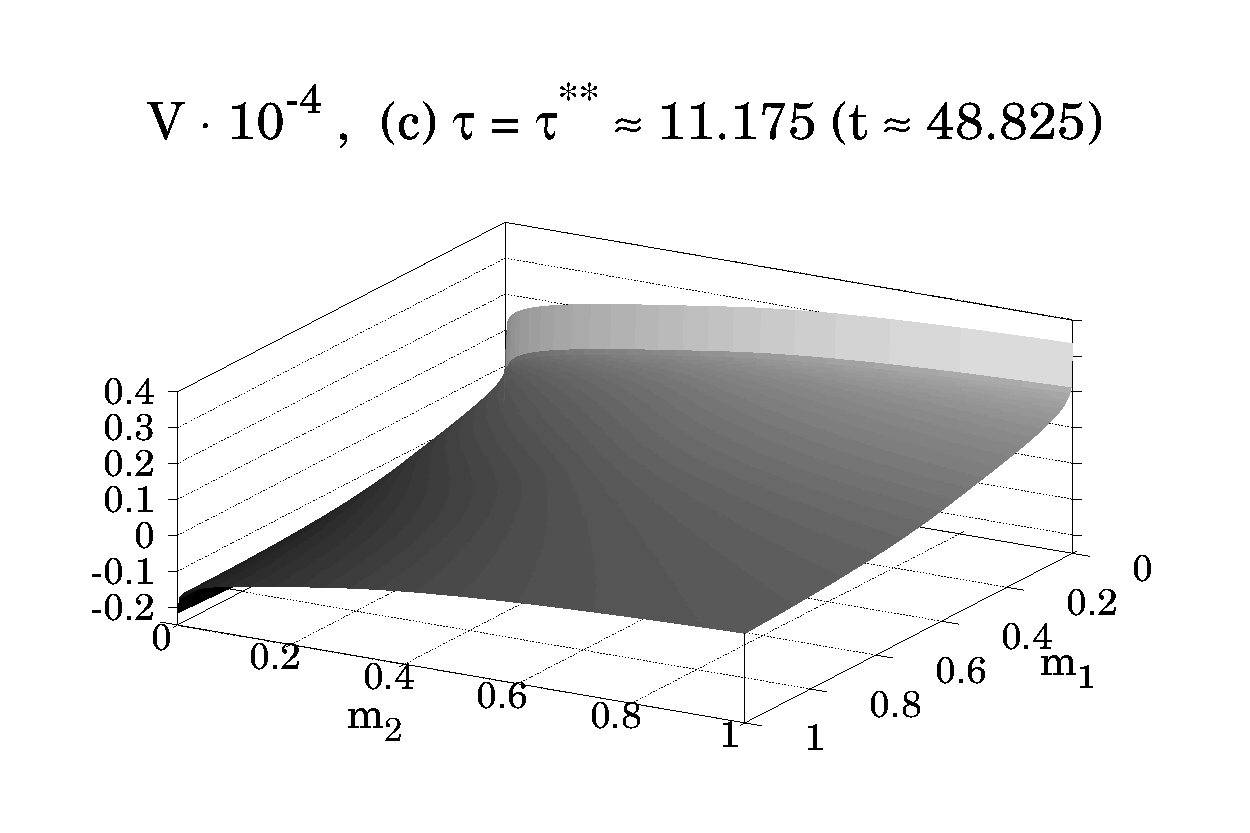
\includegraphics[width = \textwidth]{figures/Figure_4c_1.pdf}
        \caption{Competition and strategies begin to evolve.}
        \label{fig_4_c}
    \end{subfigure}
    \hfill
    \begin{subfigure}{.48 \textwidth}
        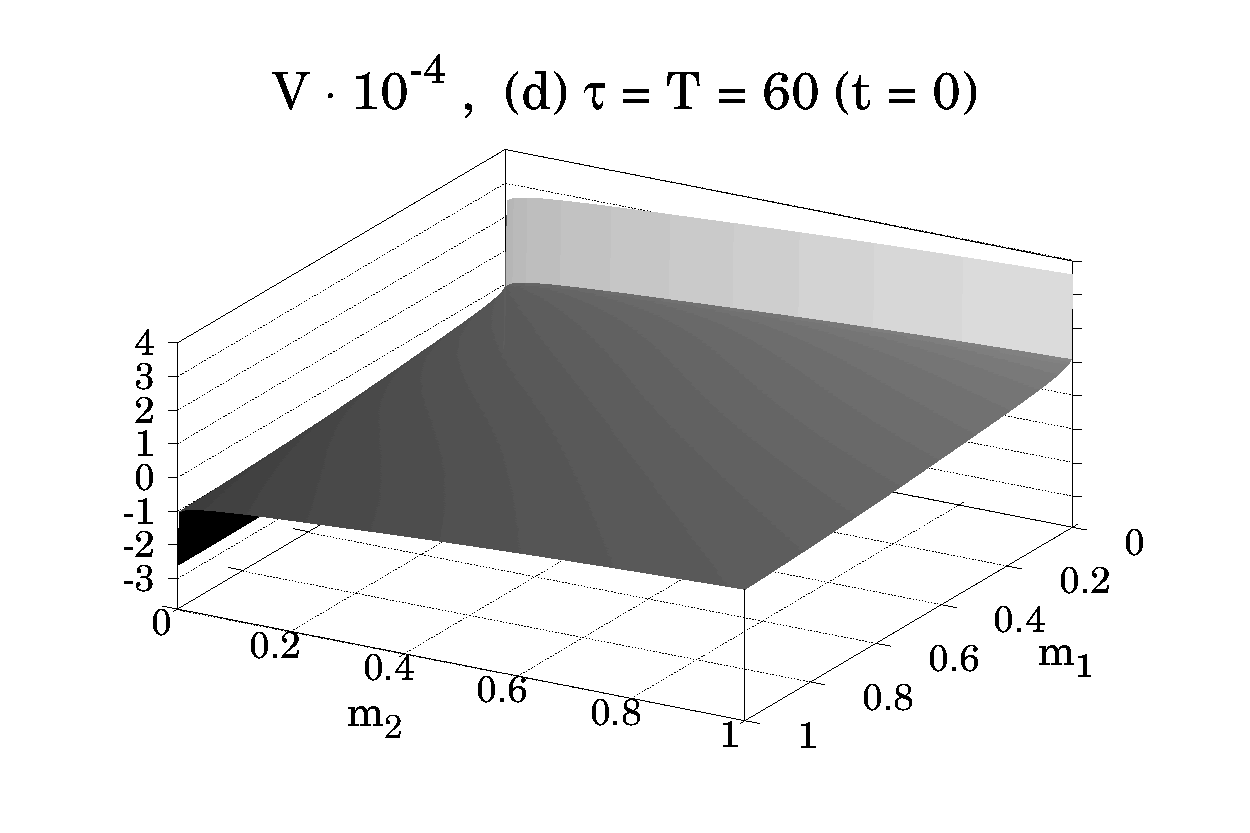
\includegraphics[width = \textwidth]{figures/Figure_4d_1.pdf}
        \caption{Strategies begin to form as the fungi take their first move.}
        \label{fig_4_d}
    \end{subfigure}

\bf \caption{\it The time instants are in reverse order to show how the computer computes the strategies using reverse time meaning the first graph is the last computation.}
\label{Fig_4}
\end{figure}
\end{frame}

% \subsection{Analysis, and Limitations}
\begin{frame}{Limitations}
    \begin{itemize}
        \item This is not super general
        \item One-seasonal
    \end{itemize}
\end{frame}

\section{Conclusion}
\begin{frame}{Conclusion}
    
\end{frame}

\begin{frame}{References}
    \bibliographystyle{plain}
    \bibliography{steven_sources.bib}
\end{frame}

\end{document}